
\begin{enumerate}
%%%%%%%%%
\item Para reconocer el estado en que esta la materia, su ordenamiento molecular está definido por la presión y temperatura a que este sometido para alejar o separar sus moléculas, llevando a ésta sustancia al estado sólido, líquido, gaseoso o plasma. El estado en el que se encuentra una sustancia a temperatura de -15$^o$C si su punto de ebullición es a 15$^o$C y de fusión es -12$^o$C es: \label{mon-1}


\begin{enumerate}[(A)]
\item Gaseoso porque sus moléculas se han separado.
\item Líquido porque sus moléculas experimentan cierto debilitamiento de sus enlaces. 
\item Líquido porque sus moléculas se han separado. 
\item Sólido porque sus moléculas están fuertemente enlazadas. 
\end{enumerate}

%%%%%%%%%%%
\item El diagrama de configuración electrónica presenta (figura \ref{fig:mon-2}) para cada nivel los subniveles y los electrones que les corresponde, como se muestra a continuación: \label{mon-2}

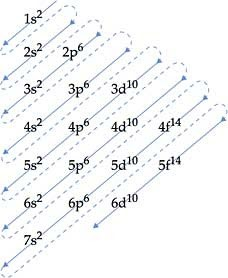
\includegraphics[width=0.35\textwidth]{imagen_0.jpg}
%\centering\captionof{figure}{Pregunta \ref{mon-2}}\label{fig:mon-2}
\justifying

Siguiendo ese diagrama para representar el siguiente átomo la configuración electrónica es:

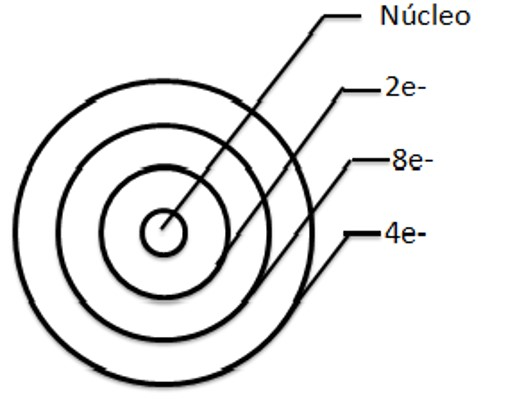
\includegraphics[width=0.45\textwidth]{imagen_1.jpg}
%\centering\captionof{figure}{Pregunta \ref{mon-2}}\label{fig:mon-2-2}
\justifying

\begin{enumerate}[(A)]
\item 1s$^2$ 2s$^2$ 2p$^6$ 3s$^2$ 3p$^4$
\item 1s$^2$ 2s$^2$ 3p$^2$ 2p$^6$ 3p$^4$
\item 1s$^2$ 2s$^2$ 2p$^6$ 3s$^2$ 3p$^2$
\item 1s$^2$ 2s$^2$ 3p$^2$ 2p$^6$ 4s$^2$
\end{enumerate}

%%%%%%%%%%%%%%
\item La estructura de Lewis es una representación de los electrones de valencia implicados en el enlace entre dos o más átomos. De acuerdo con la siguiente tabla, la estructura de Lewis que representa la molécula CO$_2$ es:\label{mon-3}


\begin{center}
\begin{tabular}{|ccc|}
\hline 
Características & C & O \\  
\hline 
Numero de e$^-$ & 6 & 8 \\ 
Numero de Protones & 6 & 8 \\ 
Numero de Neutrones & 6 & 8 \\ 
e$^-$ de valencia & 4 & 6 \\ 
\hline 
\end{tabular} 
\end{center}

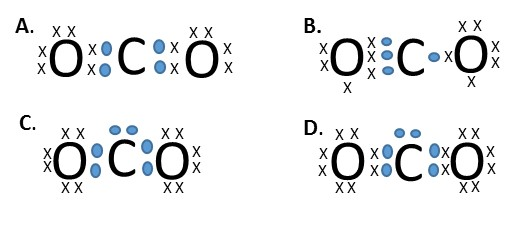
\includegraphics[width=0.45\textwidth]{imagen_2.jpg}
%\centering\captionof{figure}{Pregunta \ref{mon-3}}\label{fig:mon-3}
\justifying


%%%%%%%%%%%%%%%%%
\item La electronegatividad es una medida de la fuerza de atracción que ejerce un átomo sobre los electrones de otro y la diferencia entre las electronegatividades determina el tipo de enlace.  
En la siguiente tabla se presenta la electronegatividad de algunos elementos, por lo que el compuesto que posiblemente forme un enlace iónico es: \label{mon-4}


\begin{center}
\begin{tabular}{|ccccc|}
\hline 
Elemento & X & J & Y & L \\ 
\hline 
Electronegatividad & 4 & 1.5 & 0.9 & 1.6 \\ 
\hline 
\end{tabular} 
\end{center}
\begin{enumerate}[(A)]
\item YL
\item JL
\item YJ
\item YX
\end{enumerate}

%%%%%%%%%%%%%%%
\item Los iones, son especies químicas que han ganado o cedido electrones convirtiendo se en aniones o cationes, los aniones al ``ganar'' electrones queda con carga neta negativa y los cationes al ``perder'' electrones quedan con una carga neta positiva. El ión Cu$^{+2}$ cuenta con: \label{mon-5}

\begin{enumerate}[(A)]
\item 2 protones más que el átomo de cobre neutro.
\item 2 protones menos que el átomo de cobre neutro.
\item 2 electrones más que el átomo de cobre neutro.
\item 2 electrones menos que el átomo de cobre neutro.
\end{enumerate}

%%%%%%%%%%%%%%%%
\item Existen fuerzas al interior de los átomos de una molécula que se llaman \textbf{intramoleculares} y restando sus electronegatividades se puede conocer si se trata de un enlace iónico, covalente o metálico. Las fuerzas \textbf{intermoleculares} se refieren a atracción de moléculas para formar un estado de la materia y pueden ser dipolo-dipolo, ion-dipolo fuerzas de London o puentes de hidrógeno. Según el siguiente esquema La intensidad de fuerzas intermoleculares de los 3 estados de la materia organizada de menor a mayor es:\label{mon-6}

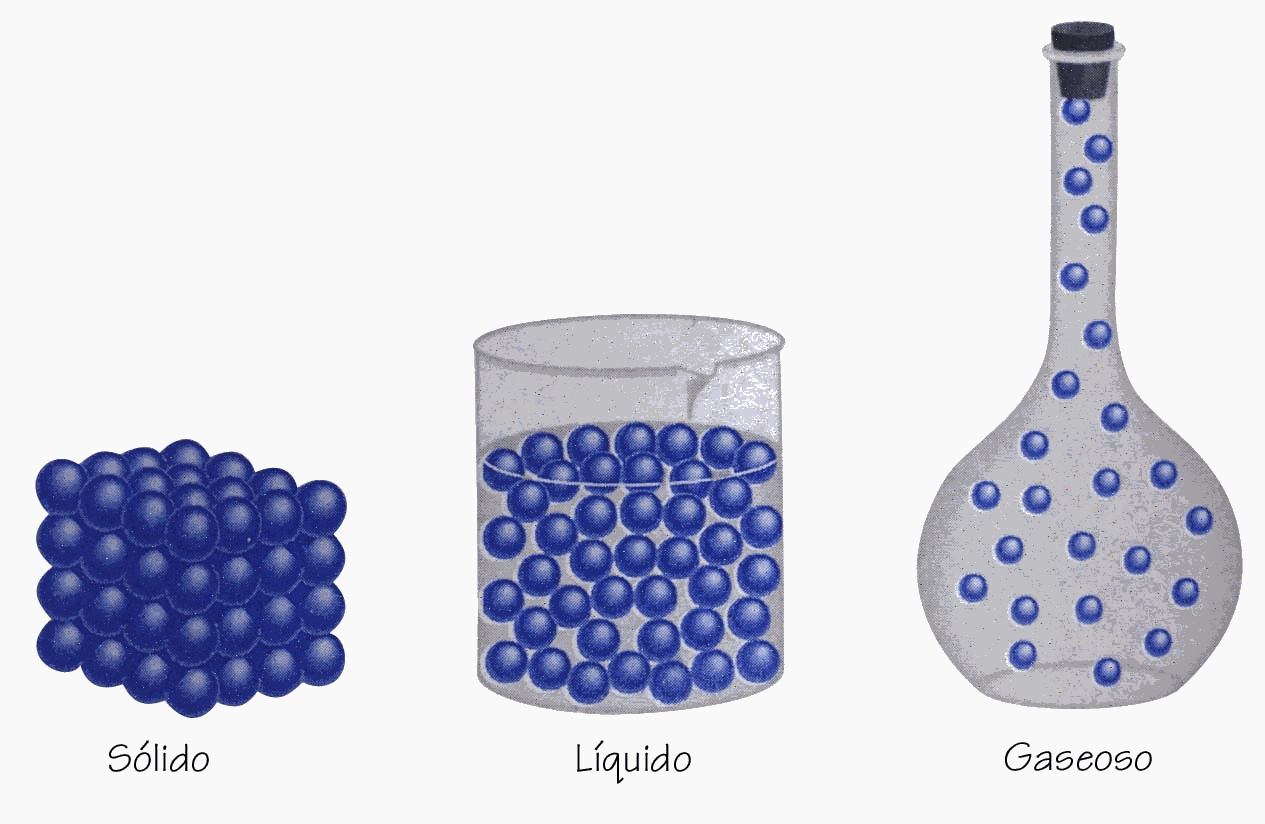
\includegraphics[width=0.45\textwidth]{imagen_4.jpg}
%\centering\captionof{figure}{Pregunta \ref{mon-3}}\label{fig:mon-6}
\justifying

\begin{enumerate}[(A)]
\item Líquido, sólido y gaseoso.
\item Gaseoso, líquido y sólido.
\item Líquido, gaseoso y sólido.
\item Sólido, líquido y gaseoso.
\end{enumerate}


%%%%%%%%%%%%%%%%
\item Con los diagramas de atómicos se identifican electrones de valencia, grupo, periodo, número atómico y por consiguiente número de electrones y protones. Además se usan las siguientes ecuaciones: \label{mon-7}

\begin{itemize}
\item Número de protones (\#p$^+$) = Número atómico (Z)
\item \#p$^+$ = Número de electrones (\#e$^-$)
\item \#neutrones = Masa atómica (A) - \#p$^+$
\end{itemize}

De acuerdo a los siguientes diagramas se presentan a continuación, una serie de afirmaciones, de las cuales NO son válidas:

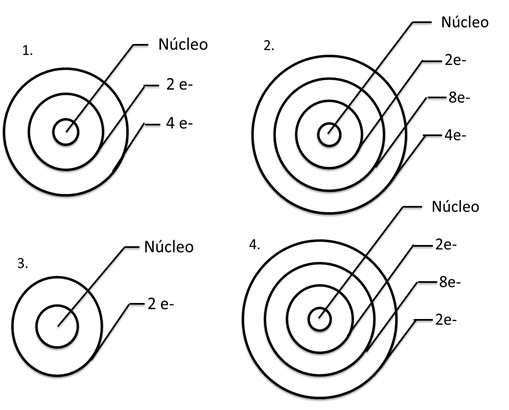
\includegraphics[width=0.45\textwidth]{imagen_5.jpg}
%\centering\captionof{figure}{Pregunta \ref{mon-3}}\label{fig:mon-7}
\justifying

\begin{enumerate}[I]
\item 1. Los diagramas 2 y 4 muestran átomos del periodo 3 
\item El diagrama 1 presenta \#e$^-$ de valencia: 4,  \#p$^+$: 6,  Z: 6, periodo:4
\item El diagrama 4 presenta \#e$^-$ de valencia: 8,  \#p$^+$: 12,  Z: 6, periodo:2
\item El diagrama 3 presenta \#e$^-$ de valencia: 2,  \#p$^+$: 2,  Z: 2, periodo:1
\end{enumerate}

\begin{enumerate}[(A)]
\item I
\item II y IV
\item I y II
\item III
\end{enumerate}


%%%%%%%%%%%%%%%%%%%%%%%%%%%
\item Una mezcla homogénea presenta una sola fase y una mezcla heterogénea dos o más fases visibles. Si se trata de una mezcla homogénea puede ser una solución cuando está compuesta de moléculas o compuestos diferentes o puede ser una sustancia pura si se compone de un solo tipo de molécula o compuesto.   El aire es una mezcla de varios gases, tales como O$_2$, N$_2$, CO, CO$_2$, CH$_4$, entre otros, por lo tanto el aire es: \label{mon-8}

\begin{enumerate}[(A)]
\item Una mezcla homogénea y sustancia pura.
\item Una mezcla heterogénea.
\item Una mezcla homogénea y solución.
\item Una mezcla heterogénea y sustancia pura. 
\end{enumerate}

%%%%%%%%%%%%%%%%%%%%%%%%%
\item La separación de una mezcla se realiza a partir de diferentes técnicas, entre éstas se encuentran: \label{mon-9}

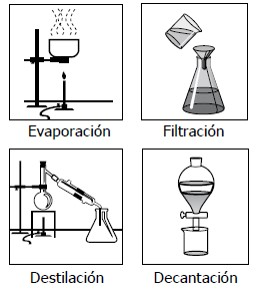
\includegraphics[width=0.45\textwidth]{imagen_6.jpg}
%\centering\captionof{figure}{Pregunta \ref{mon-3}}\label{fig:mon-7}

De éstas, la mejor técnica para desalinizar agua de mar es:
\begin{enumerate}[(A)]
\item Destilación y filtración
\item Evaporación
\item Destilación 
\item Decantación
\end{enumerate}

%%%%%%%%%%%%%%%%%%%%%%%%%%%%%%%%%%%%%%%%%%%

\item Con la destilación se separan los componentes de petróleo utilizados en las diferentes industrias a nivel mundial. En la siguiente figura se presentan los puntos de ebullición de éstos componentes, por lo que el orden en que se obtienen algunos de ellos en la destilación es:\label{mon-10}

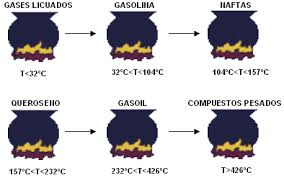
\includegraphics[width=0.45\textwidth]{imagen_7.jpg}
%\centering\captionof{figure}{Pregunta \ref{mon-3}}\label{fig:mon-7}

\begin{enumerate}[(A)]
\item Compuestos pesados, queroseno y gasolina.
\item Queroseno, gasolina y compuestos pesados
\item Gasolina, queroseno y compuestos pesados
\item Compuestos pesados, gasolina y queroseno 
\end{enumerate}

%%%%%%%%%%%%%%%%%%%%%%%%%%%%%%%%%%%%%%%%%%%%%%%
\item El astato At, es un no metal que trabaja con estados de oxidación 1,3, 5 y 7. Los ácidos se forman por la reacción de un óxido ácido y agua y las bases se forman por la reacción de un óxido básico y agua. La reacción para el ácido astático es: \label{mon-11}


\begin{enumerate}[(A)]
\item As$^{+3}$ + O$^{-2}$ $\;$ As$_2$O$_3$ + H$_2$O $\;$ As(OH)$_3$
\item As$^{+5}$ + O$^{-2}$ $\;$     As$_2$O$_5$ + H$_2$O	 $\;$  As(OH)$_5$ 
\item As$^{+5}$ + O$^{-2}$ $\;$     As$_2$O$_5$ + H$_2$O	 $\;$  H$_2$As$_2$O$_6$
\item As$^{+7}$ + O$^{-2}$ $\;$     As$_2$O$_7$ + H$_2$O	   H$_2$As$_2$O$_8$
\end{enumerate}

%%%%%%%%%%%%%%%%%%%%%%%%%%%%%%%%
\item Dependiendo de la presión y temperatura a la que se someta un material, se puede construir su diagrama de fases para observar los distintos estados de agregación. En la siguiente figura, se presentan los cambios de estado. La relación con el diagrama de fases de una sustancia desconocida que pasa del punto 1 al punto 2, experimenta los siguientes cambios de estado: \label{mon-12}

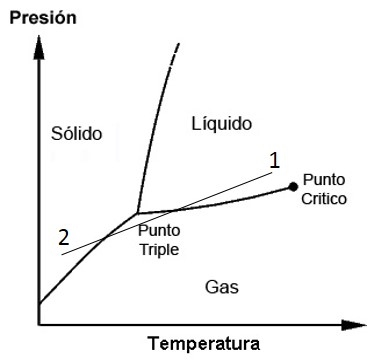
\includegraphics[width=0.45\textwidth]{imagen_9.jpg}
%\centering\captionof{figure}{Pregunta \ref{mon-3}}\label{fig:mon-7}
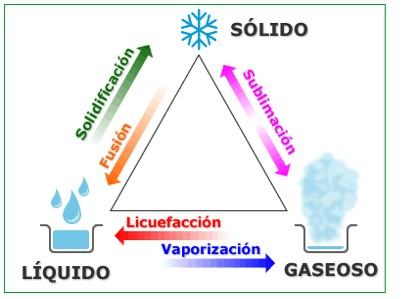
\includegraphics[width=0.45\textwidth]{imagen_8.jpg}
%\centering\captionof{figure}{Pregunta \ref{mon-3}}\label{fig:mon-7}

\begin{enumerate}[(A)]
\item Vaporización y solidificación
\item Vaporización y sublimación
\item Sublimación y licuefacción
\item Sublimación y fusión
\end{enumerate}

%%%%%%%%%%%%%%%%%%%%%%%%%%%%%%%%%%%%%%%%%%
\item La solubilidad se define como la cantidad máxima de soluto que puede disolverse en un disolvente a una presión y temperatura dada. En la siguiente gráfica se presenta la solubilidad de diversas sustancias en 100$g$ de agua y su variación con el cambio la temperatura. \label{mon-13}


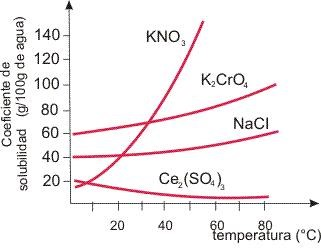
\includegraphics[width=0.4\textwidth]{imagen_10.jpg}
%\centering\captionof{figure}{Pregunta \ref{mon-3}}\label{fig:mon-7}
\begin{enumerate}[(A)]
\item Cloruro de sodio y sulfato de cesio.
\item Nitrato de potasio y dicromato de potasio.
\item Cloruro de sodio y dicromato de potasio.
\item Nitrato de potasio.
\end{enumerate}


%%%%%%%%%%%%%%%%%%%%%%%%%%%%%%%%%%%%%%%%%%
\item El magnesio es un elemento que el organismo necesita para funcionar correctamente. Su óxido es usado como antiácido, laxante o suplemento alimenticio. Se obtiene gracias a la acción del oxígeno sobre el metal con la siguiente reacción: \label{mon-14}

\begin{center}
\begin{tabular}{|cc|}
\hline 
Sustancia & Masa molar (g/mol) \\
\hline 
Mg & 24\\
O & 16 \\
\hline 
\end{tabular} 
\end{center}
\begin{equation*}
2Mg + O_2   \qquad \qquad        2 MgO   
\end{equation*}

Si existe suficiente cantidad de reactivos, para producir 10 g de MgO se necesita:

\begin{enumerate}[(A)]
\item 2.5 mol de Mg y 1,25 mol de O$_2$
\item 0.25 mol de Mg y 0,25 mol de O$_2$
\item 0.25 mol de Mg y 0,125 mol de O$_2$
\item 2.5 mol de Mg y 2.5 mol de O$_2$
\end{enumerate}

%%%%%%%%%%%%%%%%%%%%%%%%%%%%%%%%%%%%%%%%%%
\item La contaminación ambiental produce óxidos que al reaccionar con el agua de la atmosfera produce diversos ácidos, que al condensarse producen la lluvia ácida. El óxido de azufre (VI) produce ácido sulfúrico (H$_2$SO$_4$), el dióxido de carbono produce ácido carbónico (H$_2$CO$_3$). Si en una zona geográfica específica la cantidad de SO$_3$ producido genera 120 mL del ácido por cada 300mL de solución y un 56\% de concentración volumen-volumen de ácido carbónico, el ácido que más daño causa al caer por estar más concentrado es: \label{mon-15}

\begin{enumerate}[(A)]
\item El H$_2$SO$_4$ debido a que tiene un volumen mayor al de la concentración de H$_2$CO$_3$.
\item El H$_2$CO$_3$ debido a que su solución tiene un volumen menor y está más concentrado que el H$_2$SO$_4$.
\item El H$_2$SO$_4$ debido a que su concentración es mayor a la del H$_2$CO$_3$.
\item El H$_2$CO$_3$ debido a que su concentración del 56\% en comparación con el 40\% de H$_2$SO$_4$.
\end{enumerate}


%%%%%%%%%%%%%%%%%%%%%%%%%%%%%%%%%%%%%%%%%%
\item Un mol se define como la cantidad de sustancia que contiene $6,023 \times 10^{23} $ partículas, ya sea de un elemento o de un compuesto. Fue el italiano Amadeo Avogadro quien descubrió que volúmenes iguales de diferentes gases, bajo las mismas condiciones de temperatura y presión contenían igual número de moléculas. Según lo anterior, dos recipientes de igual capacidad contienen respectivamente 2 moles de N$_2$ y 2 moles de H$_2$, por lo que es válido afirmar que: \label{mon-16}

\begin{enumerate}[(A)]
\item La masa en los dos recipientes es igual.
\item  El volumen de los dos gases es igual.
\item  El número de moléculas de O$_2$ es mayor que el de N$_2$.
\item Los dos recipientes contiene igual número de moléculas.
\end{enumerate}


%%%%%%%%%%%%%%%%%%%%%%%%%%%%%%%%%%%%%%%%%%
\item La reacción F+ C  $\Longrightarrow$  Z + H se hace por duplicado y se reportan en la siguiente tabla las masas de reactivos y productos. \label{mon-17}

\begin{center}
\begin{tabular}{|ccccc|}
\hline 
Experimento & \multicolumn{2}{c}{Masa} & \multicolumn{2}{c|}{Masa}\\
 & \multicolumn{2}{c}{reactivos} & \multicolumn{2}{c|}{productos}\\ 
\hline 
 & F & C & Z & H \\ 

1 & 5 & 10 & 13 & 2 \\ 

2 & 10 & 20 & 8 & 22 \\ 
\hline 
\end{tabular}  

Según los datos reportados en la tabla es válido afirmar que se cumple la ley de la conservación de la materia porque:

\end{center}
\begin{enumerate}[(A)]
\item El número de sustancias reaccionantes es igual al número de sustancias obtenidas.
\item La masa de los productos es menor que la masa de los reactivos. 
\item La masa de los productos es igual a la masa de los reactivos.
\item El número de moles de los productos es igual al número de moles de los productos.
\end{enumerate}

%%%%%%%%%%%%%%%%%%%%%%%%%%%%%%%%%%%%%%%%%%
\item A 20$^o$C, un recipiente contiene un gas. En la siguiente figura se muestra el volumen del gas a diferentes presiones.\label{mon-18}


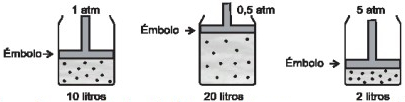
\includegraphics[width=0.45\textwidth]{imagen_11.jpg}
%\centering\captionof{figure}{Pregunta \ref{mon-3}}\label{fig:mon-7}

La grafica que mejor describe la variación del volumen cuando cambia la presión es



\begin{enumerate}[(A)]
\item 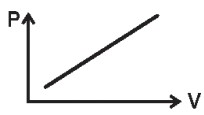
\includegraphics[width=0.4\textwidth]{imagen_12.jpg}
\item 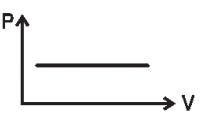
\includegraphics[width=0.4\textwidth]{imagen_13.jpg}
\item 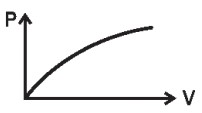
\includegraphics[width=0.4\textwidth]{imagen_14.jpg}
\item 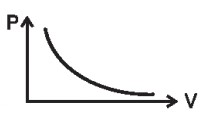
\includegraphics[width=0.4\textwidth]{imagen_15.jpg}
\end{enumerate}


%%%%%%%%%%%%%%%%%%%%%%%%%%%%%%%%%%%%%%%%%%
\item María agrega 3 cm3 de un gas a un pistón (ver figura \ref{fig:mon-19-1}). Posteriormente aumenta su temperatura sin afectar su presión (ver figura \ref{fig:mon-19-2}) \label{mon-19}

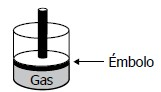
\includegraphics[width=0.4\textwidth]{imagen_16.jpg}
\captionof{figure}{}\label{fig:mon-19-1}
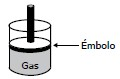
\includegraphics[width=0.4\textwidth]{imagen_17.jpg}
\captionof{figure}{}\label{fig:mon-19-2}

Desea conocer si el volumen aumentó o disminuyo de manera directa o inversamente proporcional al aumentar la temperatura. \hrulefill\\
\_\hrulefill\\
\_\hrulefill\\
\_\hrulefill.

%%%%%%%%%%%%%%%%%%%%%%%%%%%%%%%%%%%%%%%%%%
\item En el laboratorio se realizó el procedimiento que se describe en el diagrama, para identificar los cationes plata Ag$^+$, plomo Pb$^{2+}$ y mercurio Hg$^{+}$ en una muestra problema \label{mon-20}


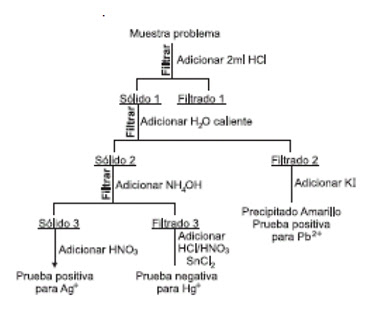
\includegraphics[width=0.45\textwidth]{imagen_18.jpg}
%\centering\captionof{figure}{Pregunta \ref{mon-3}}\label{fig:mon-7}

Durante el procedimiento se realizó una prueba de pH para cada uno de los filtrados arrojando los siguientes resultados:

\begin{enumerate}[(A)]
\item Filtrado 1 es ácido, 2 es neutro y 3 es ácido.
\item Filtrado 1 es neutro, 2 es básico y 3 es ácido. 
\item Filtrado 1 es ácido, 2 es neutro y 3 es básico.
\item Filtrado 1 es básico, 2 es ácido y 3 es neutro.
\end{enumerate}

%%%%%%%%%%%%%%%%%%%%%%%%%%%%%%%%%%%%%%%%%%
\item Durante la respiración celular se genera CO2 que se libera al torrente sanguíneo, donde puede reaccionar con agua para formar ácido carbónico, H2CO3 y contribuir, consecuentemente, al equilibrio acido - base; el proceso se ilustra mediante la siguiente serie de ecuaciones \label{mon-21}

\begin{enumerate}[(1)]
\item CO$_{2 (g)}$ + H$_2$O$_{(l)}$ $\qquad $ H$_2$CO$_{3 (ac)}$
\item   H$_2$CO$_{3 (ac)}$     $\qquad $ HCO$_{3 (ac)}^-$ + H$_{(ac)^+}$
\item  HCO$_{3 (ac)}^-$       $\qquad\ $  CO$_{3(ac)}^=$ + H$^{+}_{(ac)}$
\end{enumerate}

La siguiente tabla presenta algunas teorías del concepto ácido base.
\begin{tabular}{|p{.95in}p{2.2in}|}
\hline 
Autores & Teoría\\
\hline 
J.N Bronsted \& & \textit{Ácido}: Molécula o ion capaz de donar un protón (ion H$^{+}$) a otra sustancia. \\
T.M Lowry &\textit{Base}: Molécula o ion capaz de captar un protón (ion H$^{+}$). \\
\hline 
Gilbert & \textit{Ácido}: Molécula o ion capaz de aceptar un par de electrones libres para formar un enlace covalente. \\
\hline 
Newton  Lewis & \textit{Base}: Molécula o ion capaz de donar un par de electrones libres para formar un enlace covalente.\\
\hline 
\end{tabular} 


\begin{enumerate}[(A)]
\item 2, como una base porque tiene átomos de H en su estructura.
\item  3, como una base porque dona al medio un par de electrones libres.
\item  3, como un ácido porque libera al medio protones (iones H$^{+}$).
\item 2, como un ácido porque puede aceptar protones (iones H$^{+}$) del medio.
\end{enumerate}


%%%%%%%%%%%%%%%%%%%%%%%%%%%%%%%%%%%%%%%%%%
\item Un sistema se considera en equilibrio cuando la velocidad de formación de productos coincide con la velocidad de descomposición de éstos. Según Louis Le Chatelier, al cambiar las condiciones del equilibrio, tales como la concentración de reactivos o productos, la reacción se desplazará en la dirección que tienda a restablecer el equilibrio. Un ejemplo es la síntesis de Haber para producir amoniaco como se presenta en la siguiente reacción: \label{mon-22}
\begin{equation*}
N_2 + 3H_2 \qquad  2NH_3 
\end{equation*}

El equilibrio se modifica si se cambia la concentración de 	H2, por lo que al disminuir su concentración el equilibrio se desplaza hacía

\begin{enumerate}[(A)]
\item Los reactivos, porque se favorece la producción de N$_2$.
\item  Los productos, porque se favorece la formación de NH$_3$.
\item  Los reactivos, porque se favorece la producción de H$_2$.
\item Los productos, porque aumenta su concentración.
\end{enumerate}

%%%%%%%%%%%%%%%%%%%%%%%%%%%%%%%%%%%%%%%%%%
\item Los alcoholes primarios se oxidan hasta su correspondiente aldehído o ácido carboxílico, los alcoholes secundarios se oxidan a cetona y los terciarios no se oxidan, lo cual depende de la concentración y cantidad de oxidante. \label{mon-23}

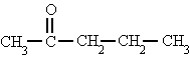
\includegraphics[width=0.4\textwidth]{imagen_19.jpg}
%\centering\captionof{figure}{Pregunta \ref{mon-3}}\label{fig:mon-7}
El alcohol del que proviene del anterior compuesto 
\begin{enumerate}[(A)]
\item 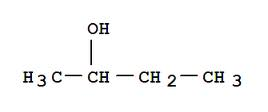
\includegraphics[width=0.4\textwidth]{imagen_20}
\item 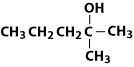
\includegraphics[width=0.35\textwidth]{imagen_21}
\item 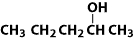
\includegraphics[width=0.35\textwidth]{imagen_22}
\item 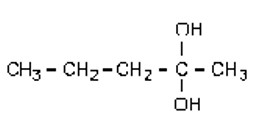
\includegraphics[width=0.4\textwidth]{imagen_23}
\end{enumerate}


%%%%%%%%%%%%%%%%%%%%%%%%%%%%%%%%%%%%%%%%%%
\item La halogenación de alquenos produce la ruptura de su insaturación, por lo que la reacción que mejor representa este proceso es \label{mon-24}


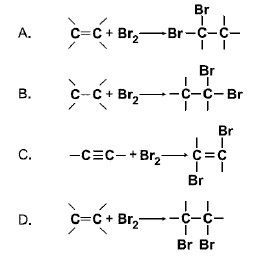
\includegraphics[width=0.4\textwidth]{imagen_24.jpg}
%\centering\captionof{figure}{Pregunta \ref{mon-3}}\label{fig:mon-7}



%%%%%%%%%%%%%%%%%%%%%%%%%%%%%%%%%%%%%%%%%%
\item La fórmula general de los alcanos es C$_n$ + H$_{2n+2}$ siendo n el número de átomos de carbono de la molécula. La fórmula para el butano es  \label{mon-25}\hrulefill\\
\_\hrulefill\\
\_\hrulefill\\
\_\hrulefill.



%%%%%%%%%%%%%%%%%%%%%%%%%%%%%
\end{enumerate}
%%%%%%%%%%%%%%%%%%%%%%%%%%%%%5


